\documentclass[11pt,a4paper]{article}
\usepackage[T1]{fontenc}
\usepackage[utf8]{inputenc}
\usepackage{lmodern,microtype}
\usepackage[margin=27mm,headheight=15pt]{geometry}
\usepackage{amsmath,amssymb,amsthm,mathtools}
\usepackage{booktabs,tabularx,longtable,array,graphicx}
\usepackage[dvipsnames]{xcolor}
\usepackage{enumitem}
\usepackage{fancyhdr}
\usepackage{tikz}
\usetikzlibrary{arrows.meta,positioning,calc}
\usepackage{listings}
\usepackage[numbers,sort&compress]{natbib}
\usepackage{xurl}
\usepackage[colorlinks=true,linkcolor=MidnightBlue,citecolor=MidnightBlue,urlcolor=MidnightBlue,
 pdfauthor={ProveIt project; prepared with ChatGPT},
 pdftitle={Signed Primitive Annuli and Compressed Basis Certificates for Unknot Hierarchies}]{hyperref}
\usepackage[capitalise,noabbrev]{cleveref}
\setlength{\parskip}{4pt}
\setlength{\parindent}{14pt}
\setlength{\emergencystretch}{2em}
\setlist{itemsep=3pt,topsep=5pt}
\renewcommand{\arraystretch}{1.18}
\newcolumntype{Y}{>{\raggedright\arraybackslash}X}
\newtheorem{theorem}{Theorem}[section]
\newtheorem{proposition}[theorem]{Proposition}
\newtheorem{lemma}[theorem]{Lemma}
\newtheorem{corollary}[theorem]{Corollary}
\theoremstyle{definition}
\newtheorem{definition}[theorem]{Definition}
\newtheorem{example}[theorem]{Example}
\newtheorem{question}{Research question}
\theoremstyle{remark}
\newtheorem{remark}[theorem]{Remark}
\newcommand{\cycred}{\operatorname{cycred}}
\newcommand{\ab}{\operatorname{ab}}
\newcommand{\bits}{\operatorname{bits}}
\newcommand{\Inn}{\operatorname{Inn}}
\newcommand{\Aut}{\operatorname{Aut}}
\newcommand{\Out}{\operatorname{Out}}
\newcommand{\code}[1]{\texttt{\small\detokenize{#1}}}
\newcommand{\complete}{\textsf{COMPLETE}}
\newcommand{\inconclusive}{\textsf{INCONCLUSIVE}}
\newcommand{\basecommit}{\texttt{e0b2f802f336fcb51e9ec5f29174cfe28dfb9d39}}
\pagestyle{fancy}
\fancyhf{}
\fancyhead[L]{\small Signed primitive annuli}
\fancyhead[R]{\small ProveIt research draft}
\fancyfoot[C]{\thepage}
\lstset{basicstyle=\ttfamily\small,columns=fullflexible,keepspaces=true,
 breaklines=true,frame=single,rulecolor=\color{black!20},
 backgroundcolor=\color{black!2},showstringspaces=false,xleftmargin=5pt,xrightmargin=5pt}

\title{\vspace{-12mm}\textbf{Signed Primitive Annuli and\\Compressed Basis Certificates\\for Unknot Hierarchies}\\[5mm]
\large Exact simultaneous recognition in rank-two support blocks,\\
source-authenticated implementation, and a research programme}
\author{ProveIt project --- research draft\\
\normalsize Prepared with ChatGPT for Vladimir Reshetnikov}
\date{12 October 2026\\[2mm]\small Repository baseline: \texttt{e0b2f802f336}}

\begin{document}
\maketitle
\begin{abstract}
We develop and implement a signed terminal rule for the compressed normal-cut
pipeline in ProveIt. After a geometrically certified core cancellation, we
retain the ordered, signed conjugacy classes of every pending annulus. We
then certify that these classes are simultaneously part of one free basis.
Gordon's primitive-loop theorem converts this algebraic certificate into
disjoint geometric dual disks, yielding an exact handlebody census.

The main algorithmic theorem is an exact polynomial-time decision procedure
for compressed cyclic families whose generator-support components have rank
at most two. In rank two, one lift of the inverse exponent-sum matrix decides
a pair: apply the lift once and test for two distinct generator conjugacy
classes. We give a self-contained subgroup-heredity proof for the block
reduction, a linear shared-grammar construction for signed transport through
column-private cancellations, and a binary-power form of backward Nielsen
replay. Classical ingredients and derived consequences are distinguished.

The implementation adds separately written source, quotient, and basis
checkers, with opt-in integration before the established whole-cut fallbacks.
Five native normal cuts that the baseline refuses acquire independently
verified certificates; Regina agrees on all five, each giving two genus-two
handlebodies. An independent literal Whitehead audit finds no disagreement
on 8,486 inputs. Compressed stress tests reach words longer than $2^{2048}$
without materializing them.

These results improve a genuine local decision stage. They do not establish
the complete quasi-polynomial unknot recognizer. We state the missing global
obligations against the announced target $2^{O((\log n)^3)}$, derive a
conditional complexity-transfer statement, and propose concrete further
questions on marked geometry, higher-rank residuals, and hierarchy search.
\end{abstract}

\vspace{2mm}
\noindent\textbf{Keywords.} Unknot recognition; compressed normal surfaces;
handlebody; primitive multicurve; straight-line program; Nielsen automorphism;
certificate verification; hierarchy complexity.
\newpage
\tableofcontents
\newpage

\section{Research outcome and the asymptotic target}
\label{sec:outcome}

\subsection{What this contribution changes}

The useful improvement is a change in what the terminal operator proves.
The existing operator can certify a pending annulus by finding a private
cocore in an already selected geometric disk system. Its unsigned crossing
counts are sufficient witnesses, but they can retain backtracking and
conjugating segments that disappear in the fundamental group. They also
describe only that disk system. A primitive family may require another one.

The new operator first authenticates the actual boundary curves, including
their traversal signs. It transports their conjugacy classes through the
certified core reduction, and asks whether there exists one common free
basis containing the resulting classes. This changes a fixed-disk-system
test into an exact algebraic test on a useful restricted class. Classical
topology then supplies the simultaneous dual disks. The algebra is applied
only after the core is known geometrically to be a handlebody.

The distinction between \emph{each curve is primitive} and \emph{the whole
family is primitive} is essential. Parallel copies of a primitive curve
pass every separate single-curve test but cannot have distinct simultaneous
dual disks. The common automorphism and distinct target letters in our
certificate enforce the family condition directly.

\begin{table}[ht]
\centering\small
\begin{tabularx}{\textwidth}{@{}p{34mm}YY@{}}
\toprule
Claim & Established here & Precise scope\\
\midrule
Signed quotient transport & Linear number of grammar productions & Complete
row-leaf or column-private source schedules; polynomial bit overhead\\
Common basis replay & Polynomial certificate verification & A supplied
powered Nielsen sequence, in any rank\\
Exact discovery & Deterministic polynomial algorithm & Cyclic support blocks
of at most two generators\\
Geometric terminal & Exact handlebody census & Authenticated core and all
pending annuli; disk interfaces allowed\\
Native improvement & Five new certified cuts & Fixed, embedded report-57
fixtures; independent replay and Regina agreement\\
Global target & Conditional accounting only & No bound proved here for
complete hierarchy discovery or repair\\
\bottomrule
\end{tabularx}
\caption{Claim ledger. Grammar size, verification, discovery, and the global
recognizer are different statements.}
\label{tab:claims}
\end{table}

\subsection{Repository baseline and relation to prior work}

All comparisons use repository revision \basecommit, whose commit message
is ``New research reports.'' The inspected sources include
\path{Topology/UnknotRecognition}, its maintained synthesis, and the
incoming reports present at that revision~\cite{proveit2026}. In particular,
the existing column-peeling theorem already decides \emph{complete positive
row cancellation in a fixed unsigned incidence matrix}. Reordering the
same positive pivots cannot defeat its stopping set. That theorem and its
sparse timestamp checker are prior ProveIt work, not results of this article.

The baseline also contains actual core-side annulus transport, a joint
bundle boundary kernel, adaptive lower forests, certified top 2--3
cancellation, and deterministic compressed word algorithms. The incoming
reports on exceptional rows, matroidal dual forests, nonlinear activation
forests, and ordered interface kernels were reviewed before choosing this
direction. A fresh search among those already covered unsigned choices
would risk reproducing existing improvements. The present extension instead
retains signs and cyclic order, then changes the free basis in a verified
handlebody. Its native fixtures are checked against the complete baseline
wrapper, including its adaptive forests and boundary-kernel fallback.

For integration, the patch preserves \code{annulus_method='counts'} as the
default and adds \code{annulus_method='signed_rank_two'}. This permits direct
comparison and preserves existing certificate formats. The experimental
option is conservative: unsupported blocks, failed primitive tests, and
exhausted resource allowances yield a refusal by this method. They never
produce a negative topological verdict.

\subsection{The published and announced complexity statements}

Lackenby's March 2021 slides state the target, for a diagram with $n$
crossings, as
\begin{equation}
 T(n)=2^{O((\log n)^3)}=n^{O((\log n)^2)}.
 \label{eq:target}
\end{equation}
The slides describe a polynomial bound on surface complexity and an
$O((\log n)^2)$ hierarchy-length bound, using efficient encoding,
multisurfaces, and Heegaard/Cheeger-region arguments~\cite{lackenby2021}.
The target is not the stronger expression $n^{O(\log n)}$.

The July 2026 paper gives a new hierarchy algorithm and explicitly leaves
possible speed-up to future work. Its Proposition 9.1 bounds iterations by
$L(g+1)^L$, where $L$ bounds hierarchy length and $g$ bounds pattern
complexity. Its Theorem 14.4 already gives polynomial-time compressed
cutting data for uniform-type handle structures, in the handle count and
the logarithm of extended surface weight~\cite{lackenby2026}. We therefore treat
compressed cutting as an established mathematical ingredient, while
assessing the particular executable ProveIt contracts separately.

The remaining problem is quantitative and constructive: maintain adequate
marked geometric information, choose useful surfaces, control discarded
suffixes after repairs, and close every terminal state required by a
complete recognizer. Faster arithmetic in one cut is useful only if those
outer operations satisfy compatible bounds. Section~\ref{sec:global} makes
this accounting explicit.

\subsection{Classical ingredients and the contribution's novelty}

The single-curve relation between primitive elements and dual disks, and
Gordon's theorem on primitive sets of boundary loops, are classical
\cite{gordon1987,wu1992,cho2020}. The rank-two fact
$\Out(F_2)\cong\mathrm{GL}_2(\mathbb Z)$ is also classical.
Kapovich's July 2026 treatment supplies the compressed single-class
rank-two algorithm and the needed uniqueness of primitive conjugacy classes
with a prescribed homology vector~\cite{kapovich2026}. Shared evaluation of
supplied automorphism sequences and compressed free reduction belong to
the established theory~\cite{schleimer2008}.

Accordingly, the pair criterion below is presented as a derived simultaneous
corollary, not a new classification of rank-two primitive elements. The
contribution is the complete chain from source-oriented annuli through
compressed quotient transport, one common basis certificate, a correct
geometric terminal, independent replay, and new native successes. The
support-block reduction and explicit source-size accounting make the
restricted algorithm precise enough to use in a larger complexity proof.

\section{Input model, signs, and proof obligations}
\label{sec:input}

\subsection{Three sizes that must remain separate}

Let $n$ be the crossing count of an original diagram, $t$ the number of
tetrahedra in a supplied triangulation, and $W$ the total number of normal
disks represented by its normal coordinates. The normal coordinates are
binary integers. A local normal-cut input size includes $t$, coordinate
bit lengths, and the combinatorial boundary data; it does not include $W$
as an explicitly expanded list.

For the signed terminal, let $L$ be the total number of signed source
passages in real and passive words after forest contraction, $r$ the total
number of surviving core generators, $p$ the number of cancelled real
rows, and $q$ the number of pending annuli. Let $S$ be a shared binary
straight-line program's number of productions plus its root-list size, and let $B$ be the total
binary size of the supplied powered Nielsen moves. Generator and node
identifiers also consume bits. These quantities refer to an authenticated
compressed cut. An estimate in $S$ is not automatically an estimate in $n$.

\begin{definition}[Shared word grammar]
A straight-line program, or SLP, is a finite acyclic directed graph with
terminal rules $A\to x_j^{\pm1}$ and concatenation rules $A\to BC$,
together with a list of roots. The empty word is permitted as a distinguished
root. Different roots may share descendants. Its structural size counts
rules and roots; its encoded size also counts references and labels.
\end{definition}

A binary grammar with $S$ rules can represent a word of length exponential
in $S$. Storing the length at every node can already use quadratic total
bits. Thus an $O(S)$ production count does not claim linear bit time or
linear bytes. We use exact integers and deterministic compressed word
operations; no probabilistic equality test is used to decide a certificate.

\subsection{Authenticated geometric state}

The enclosing ProveIt operator starts from a valid triangulation and
admissible normal coordinates under its existing compact orientable
one-torus source contract. It authenticates the compressed parallelity
decomposition and the boundary attachment skeleton. In the supported state:

\begin{enumerate}
\item Each remaining core component has a geometric cancellation certificate
proving it is an orientable handlebody, with a specified free marking.
\item Every bundle base, including every isolated base, has nonempty
boundary. Each nondisk bundle with a core interface has multiplicity one
in this source representation. Its orientable total space is a handlebody.
Isolated bundle multiplicities remain binary counts.
\item Each pending circle is the midpoint section of an actual annular
interface, with an authenticated core owner and base owner. The circles are
embedded, pairwise disjoint, and disjoint from real attaching regions.
\item Every disk-base bundle absorbed into the core contributes the real
two-handle specified by its independently checked directed source path.
\item All surviving disk interfaces and every pending annulus are accounted
for in the final incidence graph and source Euler identity.
\end{enumerate}

These are premises supplied by the existing source machinery and replayed
by the enclosing verifier. A JSON list of free-group words does not establish
them. In particular, a presentation that simplifies algebraically to a free
group is not used as a substitute for a handlebody certificate.

\subsection{Recovering signed words without losing loop directions}

Choose the authenticated forest in the core's zero/one-handle graph. Orient
each nonforest one-handle and use the signed letter $\pm(h+1)$ for crossing
handle $h$. Delete forest letters only after the path's geometric direction
has been recovered. The resulting words are the usual graph-based free
marking before the real two-handles are attached.

A crucial implementation detail is that a loop one-handle has identical
endpoint owner IDs. Comparing the start and stop \emph{owners} cannot tell
which direction it was traversed. Instead the compiler compares ordered
tetrahedron/face flags with the one-handle's source and target flags. This
applies both to annular midpoint paths and to original real attaching
cycles. The source checker reconstructs these flags independently.

After forest contraction, different choices of a path to the basepoint
change a peripheral word by conjugation. Reversing its orientation changes
it to its inverse. Both are allowed by the primitive-family definition.
Erasing signs, reordering letters, or freely reducing an unauthenticated
source path is a different operation and cannot supply the same evidence.

\subsection{What is preserved by top 2--3 cancellation}

The optional second signed schema reuses the existing geometric cancellation
of a two-handle against a three-handle. In this supported operation, all
zero- and one-handles are retained and each surviving two-handle keeps its
source cycle, with an authenticated renumbering. Hence the annular path
charts and the signed one-handle marking remain available. The verifier
first replays this reduction and only then reconstructs the signed source
packet in the reduced core.

This is a narrow statement about the established reduction. It does not
assert that arbitrary handle moves preserve source charts automatically,
and it supplies no general procedure for transporting a complete marked
boundary pattern through future disk-system changes.

% Internal theory fragment for the parent article.  Not a standalone deliverable.
% Suggested classical references:
% Gordon, Topology Appl. 27 (1987), 285--299, DOI 10.1016/0166-8641(87)90093-9.
% Hensel, J. Topol. (2021), DOI 10.1112/topo.12186, Section 4.
% Kapovich, arXiv:2607.21499v1, Sections 3.1 and 8 (23 July 2026).
% Schleimer's compressed free/cyclic reduction, cited by Kapovich.

\section{Primitive annuli from authenticated compressed multiwords}
\label{sec:primitive}

The input to this section is a geometrically authenticated handlebody core,
not an arbitrary presentation of a free group.  Its remaining annular
midpoint curves are embedded and pairwise disjoint in the boundary.  Their
words must be obtained from the signed source paths and the certified core
cancellations.  The role of algebra is to find a different disk system for
these already authenticated curves.

\subsection{A classical geometric bridge and its relative form}

An ordered family $(w_1,\ldots,w_q)$ in a free group $F_r$ is
\emph{conjugate primitive} if there is one automorphism $\Phi$ of $F_r$,
distinct basis letters $x_{j_1},\ldots,x_{j_q}$, and signs
$\epsilon_i\in\{-1,1\}$ such that $\Phi(w_i)$ is conjugate to
$x_{j_i}^{\epsilon_i}$ for every $i$.  The conjugators may differ; the
automorphism may not.

\begin{proposition}[Classical bridge, relative to disk ports]
\label{prop:bridge}
Let $H$ be an orientable handlebody of genus $r$, and let
$\beta_1,\ldots,\beta_q$ be disjoint embedded simple closed curves in
$\partial H$.  Their conjugacy classes form a conjugate primitive family
if and only if there are disjoint properly embedded disks
$D_1,\ldots,D_q$ with
\[
 |\partial D_i\cap\beta_j|=\delta_{ij}.
\]
The disks may be chosen to avoid any prescribed finite family of disjoint
disk attachment regions in $\partial H$ that is disjoint from the curves.
Consequently sufficiently thin annular neighborhoods of the curves form
a simultaneous primitive family relative to those disk regions.
\end{proposition}

\begin{proof}
We give the reduction to classical results to make the exact hypothesis
clear.  For one simple boundary curve, being a primitive element of the
free fundamental group is equivalent to possessing a dual meridian
disk~\cite[Section~4]{hensel2021}.
In particular, attaching a two-handle along it gives a handlebody of genus
one less.  These are the usual primitive-curve facts.

Suppose the classes form a conjugate primitive family.  For any subset
$J\subseteq\{1,\ldots,q\}$, attach the two-handles indexed by $J$ in
any order.  After some of these attachments, the fundamental group is the
quotient by the normal closure of the corresponding basis elements.  The
remaining indexed curves are conjugates of distinct remaining basis
elements, and hence are primitive. They remain embedded boundary curves because the original curves
were disjoint.  The one-curve result applies at every stage, so every subset
of the two-handle attachments gives a handlebody.  Gordon's theorem on
primitive sets of boundary loops~\cite{gordon1987} now supplies simultaneous
dual disks.
This use of Gordon's theorem is essential: requiring only the manifold
obtained after \emph{all} attachments to be a handlebody is a weaker
condition in general.

Conversely the dual disks have connected complement: in the graph dual to
cutting along them, the curve $\beta_i$ crosses exactly the edge indexed
by $D_i$ exactly once, so that edge is a loop.  The dual graph is connected
and all its edges are loops, hence it has one vertex.  Extend the dual disks
to a complete disk system.  In its free
basis, the word of $\beta_i$ contains its own distinguished generator once
and all the other distinguished generators zero times.  It has the form
$U_i x_{j_i}^{\epsilon_i}V_i$, where $U_i,V_i$ use only the remaining
generators.  Simultaneous Nielsen changes fixing those remaining generators
send these words to distinct basis letters, up to conjugacy.

Finally isotope the boundaries of the dual disks off the prescribed disk
regions.  An outermost arc of intersection in one of those regions can be
pushed to its boundary collar; choose outermost arcs for the whole disjoint
boundary family.  This removes intersections without changing intersections
with the $\beta_i$, since the disk regions and their sufficiently small
collars avoid those curves.  No essential meridian boundary can be contained
entirely in a disk region.  Isotopy extension carries this simultaneous
boundary isotopy to the properly embedded disks.  After taking thin annular
neighborhoods, each unique crossing becomes one spanning arc.
\end{proof}

This proposition is an application of established topology, not a new
classification theorem.  It does not assert that the disks avoid additional
\emph{annular} ports whose curves were left out of the multiword.  Such a
relative annular assertion needs an additional theorem or certificate.
Our terminal rule therefore includes every pending annulus in the relevant
core component.

\subsection{Linear grammar size for signed passive transport}

\begin{proposition}[Signed triangular source transport]
\label{prop:transport}
Suppose a geometrically verified core has a complete column-private
cancellation schedule $(r_1,g_1),\ldots,(r_p,g_p)$.  Here column-private
means that, when $r_i$ is deleted, $g_i$ occurs once in $r_i$ and zero times
in every other remaining real attaching word, counting unsigned geometric
passages.  Let $L$ be the total length of the original signed real attaching
words and the signed passive words after deletion of source-forest letters.
There is a shared straight-line program of size $O(L+r+p+q)$ representing
all final passive conjugacy classes over the $r$ surviving generators.
It can be constructed without expanding any substituted word.
\end{proposition}

\begin{proof}
Every later real attaching word contains none of the earlier pivot
generators.  Thus the donor words are unchanged source words; there is no
positive fill among the real rows.  Write the donor at stage $i$ as
\[
 W_{r_i}=A_i g_i^{\epsilon_i}B_i,\qquad \epsilon_i\in\{-1,1\}.
\]
Its relation solves to
\[
 g_i=(B_iA_i)^{-\epsilon_i}.
\]
Every generator on the right is either a later pivot or a survivor.  Process
the pivots in reverse order, replacing each such generator occurrence by a
reference to its already constructed root.  The inverse of a root is a
shared formal inverse, or can be implemented by a second grammar with
reversed products at a constant-factor increase in size.  Each original
letter contributes only a bounded number of grammar symbols.  Translate
the passive source words once using these roots.

The defining equations are triangular.  Eliminating them is an explicit
Tietze isomorphism from the source core presentation to the free group on
the surviving generators.  Since the core's handlebody status and source
paths were authenticated separately, the resulting roots represent the
actual passive curves in a free basis of that handlebody.  Binarization
preserves the stated linear bound.  In particular every expanded word has
length at most $2^{O(L+r+p+q)}$, whose binary length is polynomial.
\end{proof}

For the row-leaf shortcut, the donor at each step contains its pivot once
and only previously killed generators otherwise. Induction sends every
cancelled generator to the identity; the passive roots are obtained by one
shared deletion map. This gives the same linear structural bound.

The complete column-peeling result already in the repository allows this
schedule whenever its fixed positive cancellation matrix can be completely
cancelled.  We do not claim the same linear grammar construction for an
arbitrary positive-fill schedule.  Its new output here is the signed ordered
multiword; the existing positive transport theorem supplies numerical
incidence counts instead.

\subsection{Replay of a prescribed powered Nielsen certificate}

Use elementary Nielsen transformations consisting of inversions, swaps, and
\[
 x_i\mapsto x_i x_j^k\quad\hbox{or}\quad
 x_i\mapsto x_j^k x_i,\qquad i\ne j,\quad k\in\mathbb Z,
\]
with all other generators fixed.  Exponents are binary integers.

\begin{proposition}[Shared backward replay]
\label{prop:backward}
Let a shared input grammar have size $S$ and let a supplied sequence be
$\psi_1,\ldots,\psi_m$, applied in that chronological order, so the
resulting automorphism is $\Phi=\psi_m\circ\cdots\circ\psi_1$.
Put
\[
 B=\sum_{\text{powered steps}}\bigl(1+\lceil\log_2(|k|+1)\rceil\bigr)
   +\#\{\text{swaps and inversions}\}.
\]
All transformed input roots have one shared grammar of size $O(S+r+B)$.
The construction takes polynomial bit time; lengths have $O(S+B+1)$ bits,
apart from the encoding of generator labels. Whether this supplied sequence
carries the input roots to the specified distinct generator conjugacy
classes can then be verified using deterministic compressed free and
cyclic reduction~\cite{schleimer2008}.
\end{proposition}

\begin{proof}
Scan the sequence backwards.  Maintain roots $I_t=S_0(x_t)$ for the suffix
automorphism $S_0$ already processed.  When prepending
$\psi:x_i\mapsto x_i x_j^k$, the new composite is $S_0\circ\psi$, so
the only changed root is
\[
 I_i^{\mathrm{new}}=I_i^{\mathrm{old}}
                      (I_j^{\mathrm{old}})^k.
\]
For the left version use $(I_j^{\mathrm{old}})^kI_i^{\mathrm{old}}$.
An inversion replaces one root by its inverse; a swap exchanges two old
roots simultaneously.  Binary powering adds $O(\log(|k|+1))$ grammar nodes.
All newly appended nodes refer only to old nodes, so the construction is
acyclic.  Rebuild the original grammar once with its terminals mapped to
the final $I_t$; the original sharing is retained across every passive root.

This proves the size bound and the composition convention.  At each step
the maximum expanded generator-image length increases by at most
$1+|k|$.  Combining this product with the original grammar's exponential
length bound gives the stated bit bound.  Apply compressed cyclic reduction
to each transformed root and check that the results are distinct single
basis letters, with the permitted signs.
\end{proof}

This is a source-specific use and binary-power formulation of the standard
compressed evaluation of prescribed automorphism sequences.  The general
linear sharing principle is already present in Schleimer's work and in
Kapovich's Proposition 3.2~\cite{kapovich2026}.  It does not bound the length of a sequence that
a search must discover.

\section{An exact rank-two simultaneous terminal}
\label{sec:ranktwo}

\begin{theorem}[One homology lift decides a pair in rank two]
\label{thm:pair}
Let $u,v\in F(a,b)$ be given by straight-line programs, and let
\[
 A=\begin{pmatrix}\operatorname{exp}_a(u)&\operatorname{exp}_a(v)\\
                   \operatorname{exp}_b(u)&\operatorname{exp}_b(v)
   \end{pmatrix}.
\]
If $\det A\notin\{-1,1\}$, the two conjugacy classes are not a
conjugate primitive pair.  Otherwise choose \emph{any} automorphism
$\Phi$ whose abelianization matrix is $A^{-1}$.  Then the pair is conjugate
primitive if and only if
\[
 \operatorname{cycred}(\Phi(u))=a,
 \qquad
 \operatorname{cycred}(\Phi(v))=b.
\]
There is a deterministic polynomial-time algorithm on the compressed input
that constructs a powered Nielsen lift and performs these two tests.
\end{theorem}

\begin{proof}
Necessity of the determinant condition follows by abelianization.  If the
tuple is conjugate primitive, compose its witnessing automorphism with a
signed permutation so that its two classes go to $[a]$ and $[b]$ in the
given order.  Call the resulting automorphism $\Psi$.  Its matrix must be
$A^{-1}$.

The classical rank-two isomorphism
$\operatorname{Out}(F_2)\cong\operatorname{GL}_2(\mathbb Z)$ says that
two automorphisms with the same abelianization differ by an inner
automorphism; see the recalled proof of the classical rank-two facts
in~\cite[Proposition~8.1]{kapovich2026}.  Hence $\Phi$ and $\Psi$ have the same action on conjugacy
classes.  The two displayed tests follow.  Conversely, if those tests pass,
$\Phi$ itself witnesses conjugate primitivity.

Exponent sums are obtained by addition and sign reversal on the grammar
DAG; their bit lengths are polynomial in its size.  The Euclidean algorithm
expresses the unimodular matrix $A^{-1}$ as a polynomial-size sequence of
integer shears, row interchanges, and sign changes.  Lift these operations
to powered Nielsen transformations.  The previous proposition constructs
their shared compressed action in polynomial size.  Compressed cyclic
reduction completes the decision in polynomial time.
\end{proof}

One explicit matrix procedure first sends the first column of $A$ to
$(1,0)^\mathsf{T}$ by Euclidean row operations.  The new matrix has the
form $\left(\begin{smallmatrix}1&t\\0&\delta\end{smallmatrix}\right)$
with $\delta=\pm1$.  Invert the second row if needed, then subtract $t$
times that row from the first.  The total left multiplier is $A^{-1}$.
The shear $\left(\begin{smallmatrix}1&k\\0&1\end{smallmatrix}\right)$
is lifted, for example, by $b\mapsto ba^k$, and the other shear by
$a\mapsto ab^k$.  Keeping this column-vector convention explicit prevents
a transpose or composition-order error.

For a single class, the corresponding compressed rank-two algorithm is
already proved by Kapovich~\cite[Theorem~8.7]{kapovich2026}: test coprime exponent sums, construct a
Euclidean lift sending that vector to $(1,0)^\mathsf{T}$, and test final
cyclic length one.  The underlying rank-two fact can also be seen directly.
If a primitive element $z$ has exponent vector $(1,0)^\mathsf{T}$, choose
$\Psi$ with $\Psi(a)=z$.  Its matrix has the form
$\left(\begin{smallmatrix}1&t\\0&\delta\end{smallmatrix}\right)$,
where $\delta=\pm1$.  The automorphism fixing $a$ and sending
$b$ to $a^t b^\delta$ has the same matrix.  The two automorphisms differ
by an inner automorphism, so $z$ is conjugate to $a$.  Thus the single-class
final test is also exact for any chosen homology lift.

The pair theorem is a short simultaneous corollary of
the classical rank-two outer-automorphism fact.  Its contribution here is an
exact native annular-family terminal with a checkable common lift, rather
than a claim to a new general primitivity algorithm.

\subsection{Independent small generator blocks in arbitrary rank}

\begin{lemma}[Conjugate primitive families descend to containing subgroups]
\label{lem:heredity}
Let $A$ be a subgroup of a free group $F$, and let a finite tuple of elements
of $A$ be conjugate primitive in $F$.  It is conjugate primitive in $A$.
Here the same basis-extension definition is used if $A$ has infinite rank.
\end{lemma}

\begin{proof}
We use the standard spanning-tree construction of a free basis~\cite{kapovichmyasnikov2002}.
Choose an ambient basis containing $z_1,\ldots,z_q$ such that each given
element has the form $h_i z_i^{\epsilon_i}h_i^{-1}$.  Consider the covering
graph of the corresponding basis rose associated to $A$.  The lift of
$h_i$ from its base vertex ends at a vertex $v_i$.  Since
$h_i z_i^{\epsilon_i}h_i^{-1}\in A$, uniqueness of path lifting says
that the $z_i$-edge at $v_i$ is a loop edge.  These loop edges are distinct
for distinct $i$, since their labels are distinct.

Choose a spanning tree in the covering graph; it contains none of those
loop edges.  The usual graph basis therefore contains every based loop
$t_i z_i t_i^{-1}$, where $t_i$ is the tree path to $v_i$.  The path
$h_i t_i^{-1}$ is a loop based at the covering's base vertex and hence
represents an element of $A$.  It conjugates $t_i z_i^{\epsilon_i}t_i^{-1}$
to the original given element.  The tuple is consequently conjugate to
distinct elements of a basis of $A$, as required.  This is the covering
graph form of the relevant special case of the Kurosh theorem.
\end{proof}

\begin{theorem}[Exact recognition on blocks of at most two generators]
\label{thm:blocks}
Let $F_r$ have a specified basis partitioned into disjoint blocks
$X_1,\ldots,X_s$, each of cardinality at most two, and unused generators.
Suppose every input conjugacy class is nontrivial and has a cyclically reduced
representative over one block.  Then the whole tuple is conjugate primitive
in $F_r$ if and only if every tuple assigned to a block is conjugate
primitive in that block's free group.  This is decidable in deterministic
polynomial time on compressed words.
\end{theorem}

\begin{proof}
If every block passes, extend its witnessing automorphism by the identity
on all other blocks.  The resulting block automorphisms commute and their
product sends the whole tuple to distinct generator conjugacy classes.
For the converse apply the preceding lemma to each block free factor.

A block of rank one can contain at most one curve, whose exponent must be
$1$ or $-1$.  A block of rank two can contain at most two curves.  Use the
known compressed single-class algorithm for one and the pair theorem for
two.  More curves than the block rank fail by independence in abelianization.
Trivial input classes fail.  These tests use polynomially many calls on
polynomial-size grammars, and all primitivity-discovery calls have the same
fixed rank-two bound.
\end{proof}

An automatic version cyclically reduces each word, computes its set of
appearing generators from the grammar, and joins generators occurring in
the same support.  If every nonempty connected component has at most two
generators, these components give the required partition.  If a component
is larger, this particular exact terminal has no conclusion.  Failure of a
primitive-family test is not a negative handlebody or knot certificate.

\subsection{A strict separation from unsigned singleton criteria}

Let $\theta(a)=ab$, $\theta(b)=a$, and put
$u_n=\theta^n(a)$, $v_n=\theta^n(b)$.  This is a basis pair for every
$n$, and it admits a shared grammar of size $O(n)$.  For $n\ge4$, each
word contains each generator at least twice.  Consequently its unsigned
two-by-two incidence matrix has every entry at least two: the private
cocore test has no candidate and positive singleton cancellation cannot
start.  The simultaneous rank-two criterion accepts the pair.

This is a geometric criterion separation as well.  A handlebody homeomorphism
realizing $\theta^n$ takes two standard disjoint longitude curves to a
disjoint conjugate primitive pair. Each unsigned geometric cocore
intersection count is at least the absolute corresponding homology
coordinate, so every relevant core entry is still at least two even if
these representatives have extra backtracking. One can then attach a solid-torus
orientable interval bundle over a M\"obius band to each annulus.  Each
bundle has just one fully attached boundary and supplies no unit boundary
column: that boundary represents the square of its solid-torus generator.
Thus each new bundle column has entry two in its own row and zero in the
other. Every column total in the two-row unsigned presentation is at least
two, so the prior stopping-set theorem excludes every complete positive
cancellation in that presentation. The core-side primitive family still
gives a genus-two handlebody by the gluing formula: its reduced core genus
is zero, the two bundle genera sum to two, and the attachment graph is a
tree. An implementation claim about \emph{compressed source geometry}
requires a separately authenticated representation of those homeomorphism
images.  The word grammar by itself is not such a representation.

Two safeguards illustrate why the nonabelian and simultaneous checks remain
necessary.  The word $a^2b^3$ has coprime exponent sums but is not primitive:
its quotient group has a surjection onto $S_3$, by sending $a$ to a
transposition and $b$ to a three-cycle.  A primitive relator in $F_2$
would instead give a cyclic quotient.  In fact the pair $(a^2b^3,ab^2)$
has a unimodular exponent matrix, of determinant one, and still fails
the nonabelian test.  This last pair is an algebraic control; no source
embedding is inferred from those two words.
Also, two parallel copies of a primitive boundary curve are individually
primitive but do not form a primitive family, since their two homology
columns are dependent.  No amount of separate single-curve testing repairs
that simultaneous defect.


\section{From a common basis certificate to the whole-cut census}
\label{sec:gluing}

\subsection{The primitive-annulus gluing statement}

\begin{theorem}[Terminal gluing with a primitive core family]
\label{thm:gluing}
Suppose a finite collection of orientable handlebodies is glued along
pairwise disjoint disk and annulus interfaces by orientation-compatible
identifications. Suppose every annular interface has exactly one core
endpoint and one bundle endpoint, as in an authenticated
core/interval-bundle decomposition. Each annulus is assigned to its core
endpoint. In each core handlebody $H_v$, suppose all its incident annular
midpoint classes form one conjugate primitive family, of cardinality $a_v$.
Then every connected component of the glued manifold is a handlebody.
For a connected component of the attachment graph $G=(V,E)$ its genus is
\begin{equation}
 g(G)=\sum_{v\in V}(g_v-a_v)+|E|-|V|+1,
 \label{eq:genus}
\end{equation}
where $a_v=0$ at bundle vertices and $E$ contains both kinds of remaining
interfaces. Isolated interval bundles contribute their own genera and
binary multiplicities.
\end{theorem}

\begin{proof}
By the classical bridge, choose disjoint dual disks for all the assigned
annuli at every core vertex, avoiding the other selected annuli and the disk
ports. An annulus gluing has the standard relative handle description:
connect the two pieces by a one-handle and attach one two-handle around the
annulus. Its attaching curve meets the assigned private core one-handle
exactly once and meets the other assigned private handles zero times. Cancel
this one/two pair. The connecting one-handle remains. Because the disks and
interfaces were chosen simultaneously, all these cancellations are compatible.

After doing this for all annuli, vertex $v$ contributes a handlebody of genus
$g_v-a_v$, and every graph edge corresponds to a disk gluing or connecting
one-handle. Along a spanning tree these operations form boundary connected
sums, adding genera. Each of the remaining $|E|-|V|+1$ edges adds one genus.
This proves the topology and the formula. The primitive-family condition
also implies $a_v\le g_v$, so the reduced vertex genera are nonnegative.
An isolated orientable interval bundle over a connected bordered surface
$F$ is a handlebody of genus $1-\chi(F)$: retract the base onto a graph and
take its regular neighborhood. Each isolated copy contributes independently.
\end{proof}

The formula is already used by the baseline primitive-annulus census. The
new theorem application changes how a simultaneous family is certified.
No primitive property is required of the annulus on its opposite bundle
side: its assigned core dual disk supplies the cancelling handle.

\subsection{The Euler identity is a cross-check, not the proof}

The checker recomputes graph connectivity, owners, genus deductions, and
isolated multiplicities. It also checks
\[
 \sum_g(1-g)m_g
 =\chi(\text{core})+\chi(\text{bundles})-\chi(\text{interfaces}),
\]
where $m_g$ is the claimed number of genus-$g$ components. This can detect
certain counting inconsistencies. Exact interface coverage and ownership
are enforced separately: annular interfaces have Euler characteristic zero,
so the scalar identity alone cannot detect their omission or a changed owner.
The handlebody conclusion,
however, comes from authenticated geometric cancellations and simultaneous
primitive annuli. Euler characteristic alone cannot establish it.

\subsection{A local completeness statement and its limit}

\begin{corollary}[Exact terminal on the supported algebraic class]
\label{cor:terminal}
Assume the geometric prerequisites above, a supported complete core
cancellation, and cyclic support components of size at most two in every
core's transported annular family. With sufficient resource allowance, the
new algebraic stage decides exactly whether those families are primitive.
Whenever they are, it constructs a certificate yielding the exact whole-cut
handlebody census.
\end{corollary}

\begin{proof}
Apply the support-block theorem independently in each authenticated core.
Its positive certificates give all the families required by
\cref{thm:gluing}; replay and the graph calculation then give the census.
The exact algebraic decision is independent of expanded word length.
\end{proof}

The converse conclusion ``a nonprimitive family means the glued manifold
is not a handlebody'' is not asserted. Other geometric mechanisms can make
the full gluing a handlebody. Likewise, the primitive-family test can be
exact on its stated input class while the entire normal-cut classifier is
incomplete. The code keeps the outer status \inconclusive{} for all these
method failures.

\section{Algorithm, certificate format, and encoded cost}
\label{sec:algorithm}

\subsection{Producer stages}

The new producer is deterministic once the existing core certificate and
source forest have been selected. Its stages are:

\begin{enumerate}
\item Reconstruct signed real and passive source words and their owners.
Authenticate which real rows came from disk absorption.
\item Compile the complete core schedule into one shared quotient grammar.
The row-leaf shortcut maps its cancelled generators to the identity; the
column-private case uses reverse triangular equations.
\item Validate that every source terminal lies in the declared component
alphabet, \emph{before} free or cyclic reduction can erase it.
\item Cyclically reduce each passive root. Reject the primitive condition
if any root is empty. Build the generator-support components from the
actual reduced grammar, not from exponent sums.
\item On a rank-one block, require one class with exponent $\pm1$. On a
rank-two block, require at most two classes and run the Euclidean lift test.
A larger component is outside the supported discovery class.
\item Combine the disjoint block transformations into one move list, compile
its action backwards, and map the source grammar once. Require every final
cyclic root to be its specified positive target letter, with distinct targets.
\item Publish source evidence, component coverage, and the common basis
certificate. The enclosing operator computes the graph census only after
the whole family passes.
\end{enumerate}

Empty annular families are allowed and require an empty target list. An
unused core generator is harmless. A nonempty trivial annular class is not
primitive. Independent inversion choices can always be incorporated into
the automorphism, so the emitted target letters are positive without loss
of generality.

\subsection{Euclidean matrix convention}

Exponent-sum vectors are columns. A Nielsen move
$x_i\mapsto x_j^k x_i$ adds $k$ times coordinate $i$ to coordinate $j$.
It does not add coordinate $j$ to coordinate $i$. Thus for a first column
$(p,q)^{\mathsf T}$ with $p,q>0$, reducing $p$ by $\lfloor p/q\rfloor q$
uses a move whose \emph{target letter is $b$} and donor is $a$.

The implementation first changes signs, applies the division version of
Euclid, and interchanges the axes if necessary. If the first column has
gcd one, it reaches $(1,0)^{\mathsf T}$. In the two-column case,
unimodularity makes the other column $(s,\delta)^{\mathsf T}$ with
$\delta=\pm1$. The shear $b\mapsto a^{-s\delta}b$, followed by an inversion
of $b$ when $\delta=-1$, finishes the reduction. Every exponent is stored as
one binary integer; a quotient of size $2^b$ does not cause $2^b$ repeated
elementary steps.

\subsection{A small certificate with a broader verifier}

The algebraic certificate has fields
\begin{lstlisting}
{
  "schema": "cyclic-basis-nielsen-v1",
  "generators": [sorted positive generator labels],
  "moves": [chronological powered Nielsen moves],
  "targets": [distinct positive labels, one per input root]
}
\end{lstlisting}

It contains no claimed exponent matrix or claimed reduced word that the
checker trusts. The verifier validates the move schemas, label membership,
exact integer types, side choices, and nonzero powers. It evaluates their
action independently, then performs the terminal word checks. It does not
need the producer's support partition or Euclidean choices. In particular,
the verifier can certify a supplied primitive family in rank greater than
two, even when this producer cannot discover the certificate.

The geometric wrapper records the source packet and one such certificate
for each core component. Its source packet lists the forest, real rows,
passive attachment/base/core owners, complete cancellation schedule, and
surviving generators. Ordered component and slot coverage prevents omitting
a difficult annulus or silently moving it to another component.

\begin{table}[ht]
\centering\small
\begin{tabularx}{\textwidth}{@{}p{53mm}Y@{}}
\toprule
Schema & Role\\
\midrule
\path{signed-core-annulus-source-v1} & Source-oriented real and passive words;
conditional on the enclosing authenticated geometry\\
\path{cyclic-basis-nielsen-v1} & One automorphism carrying a cyclic family to
distinct generator classes\\
\path{signed-primitive-annuli-v1} & Complete family coverage and source
transport in every core component\\
\path{normal-cut-handlebodies-signed-annuli-v1} & Whole-cut certificate after
ordinary core and disk-absorption proofs\\
\path{normal-cut-handlebodies-signed-annuli-v2} & Same terminal after replay of
the existing top 2--3 reduction\\
\bottomrule
\end{tabularx}
\caption{New schema boundaries. Older schemas retain their original meanings.}
\end{table}

\subsection{Independent replay and the shared trust base}

The checker modules do not import the producer, its Euclidean selector, its
support decomposition, or its source compiler. The signed source checker
reconstructs the geometry in a separate implementation. The quotient checker
validates the cancellation order by deletion timestamps and source incidences,
then evaluates the signed donor recursion independently. The basis checker
uses suffix-image layers and a separate left-to-right binary-power loop.

For a column-private schedule, if $\tau(r)$ is the row's deletion time and
$\pi(g)$ the pivot time of a cancelled generator, every source occurrence
of $g$ in row $r$ must satisfy $\tau(r)\le\pi(g)$. Equality is possible
only in its own pivot row, where the occurrence count must be exactly one.
This gives one pass over source incidences, plus one pass over donor words,
instead of rescanning all rows for each pivot.

Both production and replay use the baseline \code{WordArena} for exact
compressed reduction. Hence ``independent'' does not mean two independent
implementations of every theorem in compressed-word theory. The independent
literal audit described below supplies a separate reduction and Whitehead
oracle on bounded inputs. The existing source and word kernels remain part
of the software trust base; the article's mathematical proofs do not turn
Python code into a formally verified development.

\subsection{Polynomial encoded cost}

\begin{proposition}[Cost of the local algebraic stage]
\label{prop:cost}
With integer labels encoded in binary, signed source transport, support
decomposition, exact rank-at-most-two block discovery, and verification of
the emitted certificate have deterministic polynomial bit complexity in
the authenticated source encoding. The degree does not depend on the
overall core genus. For a separately supplied Nielsen certificate, the
verification bound is polynomial in the source and certificate encodings.
\end{proposition}

\begin{proof}
The signed source theorem gives $O(L+r+p+q)$ raw grammar productions.
Inverse roots and binary products preserve a linear structural bound.
All raw lengths have polynomially many bits. Deterministic compressed
cyclic reduction gives grammars of polynomial encoded size.

For each reduced grammar node, compute support by set union and exponent
sums by integer addition. Even dense arrays cost only a polynomial factor
in $r$. Connected components and membership checks are polynomial. All
nontrivial matrix calculations occur in dimension at most two. Euclidean
division has polynomial bit complexity, and the quotients and resulting
move list have polynomial total encoding size. This is uniform over
polynomially many separate blocks.

Backward replay adds $O(r+B)$ raw productions before applying the source
grammar once. The deterministic compressed reduction theorem therefore
bounds the final checks polynomially. The independent checker stores
$O(rm)$ suffix-image references for $m$ moves; this is polynomial, although
less economical than the producer's mutable image map. Integer lengths,
reference sorting, and component bookkeeping are charged in the encoded
bound. No step iterates over the expanded passive word length.
\end{proof}

The implementation's resource limits are operational guards, not asymptotic
claims: by default the new word arenas allow $10^6$ nodes and $10^7$
charged abstract operations. Python dictionary access is not being asserted
to have deterministic worst-case constant time against adversarial labels.
Ordered maps or sorted arrays can realize the polynomial theoretical
bound. The current source adapters also scan one-handles separately for
each core component, which can cost quadratic structural work. The
measured wrapper still has the source-query, forest,
normal-surface, and geometric verification costs of its existing stages.

The uniformity in rank uses the compressed free/cyclic reduction and
composition-system results, not just a fixed-group automorphism word
problem: see Schleimer's Theorem 3.3, Corollary 3.6, and
Theorem 7.1~\cite{schleimer2008}. Renumber the occurring letters; their
number is bounded by the input's terminal productions. The algorithms
operate on symbolic equality, involution, and compressed prefix comparison,
so label bits can be charged without introducing a degree depending on
the ambient rank. Initial cyclic reduction may involve the full alphabet;
only the subsequent primitivity discovery is blockwise rank two.

\section{Native evidence and reproducible experiments}
\label{sec:experiments}

\subsection{An actual signed obstruction in the discovery bank}

The first new case is \path{finite_figureEight/vertex71}, from the standard
vertex surfaces of report 57's discovery corpus at the pinned revision.
Its triangulation has ten tetrahedra and its normal coordinates represent
thirty disks. The embedded fixture includes the exact gluing permutations,
all coordinates, and the SHA-256 of the source bank. Thus reproduction does
not depend on a surface enumeration library returning the same ordering.

The baseline authenticates a complete augmented core but refuses the
remaining annuli with reason \code{annular_core_attachment}. On the relevant
core component, label the surviving generators $a=29$, $b=39$ and the
disk-absorption generator $z=55$. The two authenticated passive source words
are
\[
 z a^{-1}b^{-1},\qquad z^{-1}b^{-1}a^{-1}b.
\]
The genuine absorbed disk supplies the real row $z$, so the core quotient
sets $z=1$. The residual conjugacy classes are therefore represented by
\begin{equation}
 u=a^{-1}b^{-1},\qquad v=a^{-1}.
 \label{eq:nativepair}
\end{equation}
Their exponent-sum matrix is
\[
 A=\begin{pmatrix}-1&-1\\-1&0\end{pmatrix},\qquad \det A=-1.
\]
The emitted chronological moves invert $a$, invert $b$, send
$b\mapsto a^{-1}b$, and interchange $a,b$. Their effect on the two cyclic
representatives is visible without a large computation:
\[
 (a^{-1}b^{-1},a^{-1})
 \longmapsto (ab^{-1},a)
 \longmapsto (ab,a)
 \longmapsto (b,a)
 \longmapsto (a,b).
\]
The certificate checks the unabridged source paths, rather than accepting
these displayed shortened words as evidence.

There are two core handlebodies of genus two. One has no pending annuli;
the other meets an annulus-base interval bundle, a genus-one handlebody,
along its two boundary annuli. For the connected attached part,
\cref{eq:genus} gives
\[
 (2-2)+1+(2-2+1)=2.
\]
The isolated core contributes the other genus-two component. An independent
Regina construction cuts the actual triangulation into 297 tetrahedra and
recognizes exactly two genus-two handlebodies.

\begin{figure}[ht]
\centering
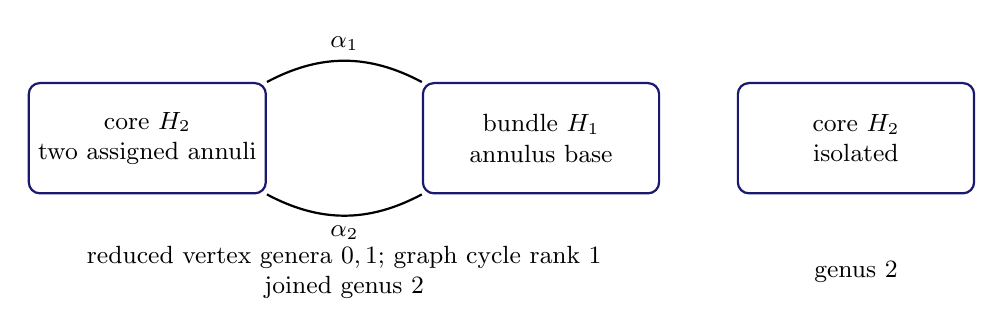
\begin{tikzpicture}[every node/.style={font=\small},
 core/.style={draw=MidnightBlue,thick,rounded corners,align=center,
               minimum width=30mm,minimum height=14mm}]
\node[core] (h) at (0,0) {core $H_2$\\two assigned annuli};
\node[core] (b) at (5,0) {bundle $H_1$\\annulus base};
\node[core] (j) at (9,0) {core $H_2$\\isolated};
\draw[thick] (h.north east) to[bend left=28] node[above] {$\alpha_1$} (b.north west);
\draw[thick] (h.south east) to[bend right=28] node[below] {$\alpha_2$} (b.south west);
\node[align=center] at (2.5,-1.7) {reduced vertex genera $0,1$; graph cycle rank $1$\\
joined genus $2$};
\node at (9,-1.7) {genus $2$};
\end{tikzpicture}
\caption{The first native gain's attachment graph. Both parallel edges
must be included in the simultaneous primitive family.}
\label{fig:native}
\end{figure}

This is a cut in a figure-eight exterior. A handlebody census of a chosen
cut is not an unknot verdict. A nontrivial knot can admit a cut into
handlebodies; the hierarchy's boundary patterns and the surface's role still
matter. The example validates the local source-to-census inference and its
strict success-set improvement.

\subsection{Further native gains, retained refusals, and the audit denominator}

The extended report-57 scan contains 1,374 standard vertex surfaces,
excluding its Fibonacci and connected-sum records. The baseline completes
1,205 and refuses 169. The recorded baseline refusal reasons are 52 raw
cancellation stalls, 101 boundary-kernel stalls, five raw ball-cancellation
obstructions, and eleven annular attachments. Inspecting the refused cases
under the tested source, maximum-passage, and reverse-ID forests finds 52
with a complete augmented core and pending annuli. Exactly five of those
families pass the signed common-basis test. All five now pass the complete
source-authenticated wrapper with its production forest policy.

\begin{table}[ht]
\centering\small
\begin{tabular}{@{}lrrrrrr@{}}
\toprule
Case & $t$ & $W$ & Source letters & Word nodes & Moves & Regina cut $t$\\
\midrule
E71 & 10 & 30 & 45 & 16 & 4 & 297\\
I134 & 13 & 37 & 56 & 24 & 2 & 377\\
I136 & 13 & 37 & 59 & 18 & 3 & 386\\
I205 & 13 & 38 & 57 & 19 & 3 & 398\\
I290 & 13 & 38 & 57 & 21 & 2 & 398\\
\bottomrule
\end{tabular}
\caption{Five new native gains. E denotes \texttt{finite\_figureEight}; I
denotes \texttt{finite\_figureEight\_interior}; numbers are the frozen
standard-vertex indices. Every result is two genus-two handlebodies, with
independent whole-cut replay and Regina 7.4 agreement.}
\label{tab:native}
\end{table}

E71 uses the ordinary signed schema. I134, I136, I205, and I290 first use
the established top 2--3 reduction and the second signed schema. The five
complete certificate files have canonical sizes 144,704; 199,262; 160,239;
198,738; and 198,726 bytes respectively. Most evidence is the existing
source geometry, rather than the short Nielsen move list.

In one recorded run, whole-cut production took between 0.053 and 0.105
seconds on these five cases, and full independent replay between 0.075 and
0.118 seconds. These are single-run observations on a shared execution
host, not an isolated timing comparison or a claimed multiplicative speed-up.
The baseline timings measure refusals; the new timings measure completed
certificates. Source encodings and exact operation counts are the more
reproducible performance evidence.

Two other exploratory banks produced no new opportunities: all 660 tested
Fibonacci vertex/scaled cuts and all 1,700 deterministic seed relabelings
were already completed by the baseline. The broader 1,374-case discovery
search took 562.07 seconds and included a separate literal Whitehead search
used to investigate refused states. That exploration time is not the cost
of the new compressed production algorithm.


The discovery procedure also retains a negative control whose transported
annular word is $x^5y^2$. It has coprime exponent sums, but it is not
primitive: the one-relator quotient maps onto $C_5*C_2$, which is nonabelian,
whereas quotienting $F_2$ by a primitive element gives an infinite cyclic
group. The new method still refuses this cut. This is a failure of the
primitive terminal, not a proof about the topology of the entire cut.

No recognition-rate claim is based on pooling the historical banks,
relabelings, and new fixtures as independent random observations. Relabelings
test invariance and exposure, while related normal surfaces can be strongly
correlated. The frozen JSON files record each exploration's denominator,
reason counts, and positive cases separately.

All five gains were also replayed with the public default
\code{boundary_method='masks'}, in addition to the recorded moments-based
run. Thus the new terminal also works with the default boundary setting.

\subsection{An independent algebraic oracle}

The independent audit enumerates all sixteen rank-two type-II Whitehead
maps and repeatedly decreases the \emph{total cyclic length} of a tuple.
It accepts exactly when a length-minimal tuple consists of distinct
one-letter classes. This uses the classical Whitehead minimization
principle; the audit's literal free/cyclic reductions and substitutions do
not import the producer, its determinant test, or \code{WordArena}.
General explicit-input minimization already has fully polynomial algorithms
in length and rank~\cite{roig2007}; the tiny exhaustive oracle is used for
independence, not as a new efficient algorithm.

\begin{table}[ht]
\centering\small
\begin{tabularx}{\textwidth}{@{}Yr r@{}}
\toprule
Decision family & Inputs & Positive\\
\midrule
Nonempty cyclically reduced rank-two words, length at most six & 1,104 & 196\\
Ordered pairs, nonempty and total cyclic length at most six & 6,576 & 648\\
Random unstructured singleton/pair inputs & 400 & 41\\
Random automorphic images with independent conjugations/inversions & 397 & 397\\
Named controls & 9 & 2\\
\midrule
Total & 8,486 & 1,284\\
\bottomrule
\end{tabularx}
\caption{Independent algebraic audit, seed 20261012. There were zero
decision discrepancies and every positive certificate replayed correctly.}
\label{tab:audit}
\end{table}

Additionally, 396 supplied Nielsen sequences in ranks two through five
matched explicit forward substitution on 4,008 unreduced outputs, with
4,008 inverse roundtrips. The largest literal output had 36,687 letters.
The sequences cover both multiplication sides, both exponent signs,
inversions, swaps, and powers of absolute value greater than one.

All 71 malformed certificate mutations were rejected. Among 24
syntactically valid alterations, twenty were invalid proofs and rejected;
four remained valid proofs and were accepted, exactly as the independent
literal replay predicted. This distinction avoids the incorrect test rule
that every changed certificate must fail. Three attempted random positive
generations and six compiler generations exceeded the \emph{literal
oracle's generation caps before testing}; they are reported as such rather
than counted as production failures. The audit ran in 6.514 seconds on the
recorded environment. Finite tests support implementation confidence; they
do not prove the asymptotic theorem.

\subsection{Compressed stress tests}

The benchmark uses four reproducible families. For the Fibonacci family,
$(u_n,v_n)=(\theta^n(a),\theta^n(b))$ with $\theta(a)=ab$, $\theta(b)=a$;
its total expanded length is $F_{n+3}$ when $F_0=0,F_1=1$. The shear family
is $(a,a^{2^b}b)$, with total length $2^b+2$. Independent support blocks use
disjoint copies of the depth-eight Fibonacci pair. The triangular source
family has relations $g_i=g_{i+1}^2$, ends at $b$, and passive word $ag_0$,
so its final length is $2^d+1$.

These are explicitly algebraic inputs. The triangular packets test the
quotient compiler, not source geometry, and no knot diagram or embedded
normal surface is inferred from them. Every positive result is independently
replayed in a freshly built word arena.

\begin{table}[ht]
\centering\small
\begin{tabular}{@{}lrrrrrr@{}}
\toprule
Family & Parameter & $\bits(N)$ & Input DAG & Final DAG & Produce ms & Verify ms\\
\midrule
Fibonacci pair & 128 & 90 & 130 & 773 & 2.57 & 2.23\\
Fibonacci pair & 2,048 & 1,423 & 2,050 & 12,293 & 41.63 & 34.69\\
Binary shear pair & 128 & 129 & 131 & 264 & 1.32 & 0.99\\
Binary shear pair & 2,048 & 2,049 & 2,051 & 4,104 & 17.54 & 12.65\\
Triangular transport & 128 & 129 & 131 & 265 & 0.72 & 0.74\\
Triangular transport & 2,048 & 2,049 & 2,051 & 4,105 & 12.16 & 12.70\\
Independent blocks & 16 & 11 & 160 & 848 & 2.82 & 2.25\\
Independent blocks & 64 & 13 & 640 & 3,392 & 11.85 & 10.75\\
\bottomrule
\end{tabular}
\caption{Selected compressed benchmarks; all positive results independently
verified. Parameters are depth $n$, exponent-bit parameter $b$, transport
depth $d$, and number of blocks, respectively. $N$ is total expanded root
length, with $\bits(N)=\lfloor\log_2N\rfloor+1$. No expanded words were
materialized. Full measurements and code hashes are in the JSON.}
\label{tab:compression}
\end{table}

\begin{figure}[ht]
\centering
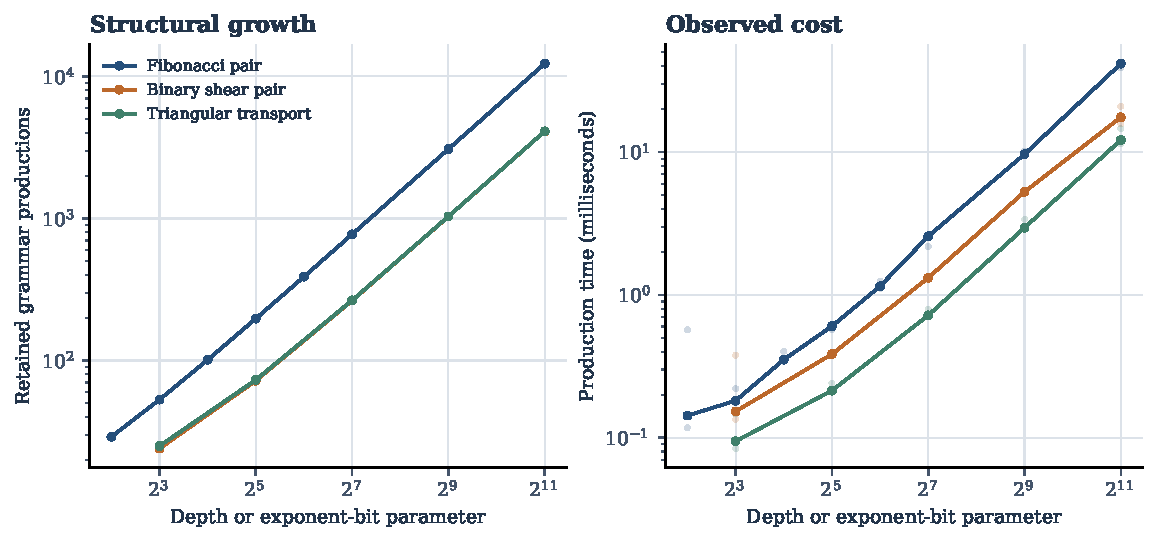
\includegraphics[width=\textwidth]{../figures/compression.pdf}
\caption{Recorded grammar sizes and elapsed production time for three
compressed families. The horizontal parameter controls exponentially large
expanded words. Straight-line growth of stored grammar sizes on these
examples illustrates the proved sharing mechanism; the finite timing curves
do not establish an asymptotic exponent.}
\label{fig:compression}
\end{figure}


Times are medians of three runs. Production time excludes construction of
the input grammar, and verification time excludes its reconstruction;
separate construction timings are stored in the JSON. Grammar counts
include arena nodes retained after processing, while the input column counts
only reachable source productions. The theoretical statements concern all
valid compressed inputs in the supported class, not an extrapolation of
these particularly structured families.

\subsection{Repository regression and reproducibility limits}

All 1,741 collected repository tests were exercised successfully: 1,733
passed in the final full run, together with 1,750 passing subtests; eight
tests were blocked at setup by a missing historical synthesis fixture and
passed in a separate 0.99-second run after its exact restoration. The full
run took 506.68 seconds and had no assertion failures. The focused suite
contains eighteen new tests covering algebra, signed source reconstruction,
and whole-cut integration.

The frozen logs preserve the setup failures rather than presenting them
as one uninterrupted green invocation. An earlier run also encountered
workspace exhaustion, a missing historical commit, and two stale refusal
expectations. Those two expectations already failed against the untouched
baseline because adaptive forests now complete the examples. They are
pinned to \code{lower_forest='source'} in the patch, preserving the
historical obstruction each test was intended to exercise. No production
behavior was changed to satisfy those assertions.

The included snapshot supports the eighteen focused tests, the native
fixtures, and the algebraic audits without a full repository checkout.
Replaying the entire upstream suite requires its original report and
synthesis fixtures and one historical commit; the README records those
dependencies. Regina is needed only for the optional expanded-cut
cross-check. These dependency boundaries are separate from the mathematical
and certificate correctness claims.

\section{What would suffice for the global quasi-polynomial bound?}
\label{sec:global}

\subsection{A quantitative transfer statement}

The following elementary consequence of a hierarchy iteration bound is a
useful specification for the remaining programme. It isolates the exact
quantities a local performance result must feed.

\begin{proposition}[Conditional hierarchy accounting]
\label{prop:global}
Consider a \emph{complete and correct} hierarchy recognizer on diagrams of
$n\ge2$ crossings, with $L(n)\ge1$, $g(n)\ge0$, and $B(n)\ge2$.
Suppose it executes at most $L(n)(g(n)+1)^{L(n)}$
iterations, and each iteration, including discovery, repairs, and terminal
work, takes at most $B(n)^d$ bit operations for a fixed constant $d$.
Assume its combined preprocessing and postprocessing also take at most
$B(n)^d$ bit operations.
Then
\begin{equation}
 \log_2 T(n)\le \log_2 L(n)+L(n)\log_2(g(n)+1)
                    +d\log_2 B(n)+O(1).
 \label{eq:account}
\end{equation}
In particular, if $L(n)=O((\log n)^2)$, $g(n)=n^{O(1)}$, and
$\log B(n)=O((\log n)^3)$, the recognizer has the bound in
\cref{eq:target}. Polynomially sized states and polynomial local work are
a stronger sufficient version of the last hypothesis.
\end{proposition}

\begin{proof}
Multiply the number of iterations by their worst-case bit cost. The
preprocessing and postprocessing cost at most one extra iteration bound,
so the total is at most $2L(n)(g(n)+1)^{L(n)}B(n)^d$.
Take base-two logarithms. The stated growth assumptions make every term on the
right $O((\log n)^3)$. This counts repeated repairs and discarded work only
because they were expressly included in the iteration and local-cost
hypotheses. Ignoring them would invalidate the bound.
\end{proof}

The proposition is a conditional accounting lemma, not a derivation of the
missing hypotheses. It is compatible with Lackenby's stated iteration
analysis and announced speed-up mechanism, but does not claim to reconstruct
that unpublished quantitative argument. The polynomial terminal in this
article helps satisfy one local-cost obligation when its structural
preconditions occur.

\subsection{Why certificates alone do not supply the search bound}

A short certificate can be easy to verify and hard to discover. Backward
Nielsen replay controls the size of the action of a \emph{supplied} sequence;
it does not control how many transformations a search tries. Likewise, a
primitive-family certificate proves the existence of a disk system without
constructing its full boundary embedding for use by a later hierarchy.

In rank two, the abelianization map resolves the discovery problem because
its outer kernel is trivial. In rank at least three this simplification
fails even for a very elementary family. In $F(a,b,c)$ the automorphism
\[
 a\longmapsto a[b,c],\qquad b\longmapsto b,\qquad c\longmapsto c
\]
has identity abelianization. The tuple $(a[b,c],b,c)$ is a basis, but the
identity lift of its homology matrix leaves a cyclic word of length five.
Thus the rank-two ``choose any lift'' argument cannot be extended by merely
enlarging the matrix. Nontrivial IA automorphisms remain to be found.

Similarly, compressed Whitehead \emph{minimality testing} and compressed
Whitehead \emph{minimization} are distinct tasks. The former asks whether a
shortening move exists at the current state; the latter follows enough moves
to reach an orbit minimum. The number of strict decreases can be governed
by the enormous expanded length. Kapovich explicitly distinguishes these
issues for compressed words~\cite{kapovich2026}. A sequence of polynomial
steps is not a polynomial algorithm without a polynomial step count.

\subsection{Marked geometry is the next interface}

The current output records a topology type and a source-valid primitive
family. A complete hierarchy may need a description of where every old
pattern edge, disk interface, and new meridian lies after the basis change.
An automorphism of the free group records none of those intersections by
itself. Handlebody homeomorphisms can act identically on the free group up
to inner automorphism while affecting boundary data~\cite{hensel2021}. The marked problem
therefore has strictly more information to carry.

A productive next representation would maintain a compressed boundary
diagram with a rotation system, local source charts, and shared path
expressions. A basis certificate would be accompanied by a checked
realization of the elementary moves on that diagram. Such a representation
must prove that its encoded size remains controlled through repeated
composition, including substitutions caused by geometric repairs. This is
an explicit research obligation, not an automatic consequence of the SLP
word bound.

\section{Further research questions and proposed approaches}
\label{sec:questions}

The questions below are ordered by the value of a concrete answer to the
existing implementation. Each states an object to construct or a bound to
prove, and an experiment or obstruction that can make progress measurable.
They are proposals, not asserted theorems.

\subsection{From terminal existence to usable marked geometry}

\begin{question}[Compressed realization of the dual disks]
Given authenticated annular source curves and a polynomial-size common
Nielsen certificate, can one construct a comparably sized certificate of
the simultaneous dual disks, together with their intersections with a
prescribed boundary pattern?
\end{question}

A first restricted target is one rank-two block in a core with only disk
ports. Maintain the boundary diagram of each Nielsen move as a local
band-slide operation, then share repeated bands using a grammar. A proof
must bound both the combinatorial chart count and the bit lengths of
repeated traversals. The decisive test is whether the resulting object can
serve as input to the next authenticated normal-cut or pattern operation.

\begin{question}[Primitive families relative to omitted annular ports]
What additional certificate characterizes a primitive subfamily whose dual
disks must avoid a specified collection of unselected annular ports?
\end{question}

The present theorem only removes disk ports freely. Relative cyclic data
could be encoded by a free-factor system or a peripheral multiword, but
the algebraic condition must be proved equivalent to the required embedded
relative disks. An initial search should look for pairs of boundary
embeddings with identical unmarked free-group data but different relative
disk behavior. Such examples would identify exactly which marking data
cannot be discarded.

\subsection{Larger algebraic blocks without expanded descent}

\begin{question}[Homology normalization followed by sparse IA correction]
After using integral row operations to normalize the homology of an
annular family, can the remaining IA obstruction be eliminated efficiently
when it is supported on a sparse interaction graph?
\end{question}

One proposed procedure checks that the homology columns span a direct
summand, completes them to an integral basis, and lifts the resulting
unimodular matrix to powered Nielsen transformations. It then studies the
residual words with unit homology. The rank-three example $a[b,c]$ shows
what this second phase must detect. A promising precise restriction is
that each residual conjugation or commutator involves a bounded-size
separator of the interaction graph. The proof target is a bound on the
total \emph{binary size} of corrections, not merely on their individual
evaluation cost.

\begin{question}[Support decomposition after certified basis changes]
Can one find a short sequence of basis changes that separates a given
family into blocks of rank at most two, or certify a useful obstruction to
such a sequence under a specified budget?
\end{question}

The current general verifier can already check the concatenation of a
supplied preliminary basis change and the exact block certificates. This
permits exploration without enlarging the trust base. A search could try
weighted Whitehead cuts or forest-induced changes, minimizing the largest
support component before minimizing length. Completeness must not be
claimed from this heuristic objective: a primitive family always admits
some basis with singleton supports, so unrestricted optimization already
contains the difficult discovery problem.

\begin{question}[Polynomial compressed minimization for native geometric
families]
Does the annular origin of the multiwords force a quantitative restriction
on Whitehead descent that arbitrary compressed free-group words lack?
\end{question}

The useful hypothesis should refer to the authenticated source embedding,
the handle structure's uniform type, or the topology of the interval-bundle
bases. Bounds expressed only in the SLP size are the general compressed
problem again. A first experiment should measure strict decreases, plateau
moves, and peak grammar size on the remaining native annular refusals, and
retain the full source certificates for any apparent structural pattern.

\subsection{Stronger source transport and terminal coverage}

\begin{question}[Signed transport beyond no-fill core schedules]
Can arbitrary certified positive-fill or geometric disk-slide schedules
be compiled into a polynomial shared signed peripheral grammar without
rebuilding every passive root at every step?
\end{question}

The column-private theorem works because the real donors remain original
source words. For general schedules one should record donor expressions as
shared definitions and maintain a persistent substitution circuit. The
main obstruction is composition: blindly substituting a new circuit into
every old circuit may destroy the desired bound. A successful theorem must
control the combined DAG and its integer lengths, as the backward Nielsen
argument does for automorphisms.

\begin{question}[Mixed core-side and bundle-side primitive families]
Can compatible partial families on both sides be combined with the signed
terminal without an exponential assignment search?
\end{question}

The baseline joint boundary kernel already handles substantial mixed
unsigned behavior. A new result must therefore use information that it
does not already capture. One possibility is a compatibility graph whose
vertices are \emph{certified simultaneous} primitive families, with edges
encoding which interfaces can share a disk system. Whether this graph has
a matroidal or bounded-width structure must be proved from the geometry;
choosing each annulus's preferred side independently is unsound.

\begin{question}[A broader exact local terminal]
Which native handlebody gluings fail primitivity on both sides but admit a
different short geometric certificate?
\end{question}

The retained $x^5y^2$ case is a useful starting point because it defeats a
specific primitive inference while keeping its provenance fixed. The
next step is to inspect a Regina disk system in the actual cut and translate
its mechanism into an elementary source-checkable move. Algebraic
freeness, homology, or a successful external recognition call alone should
not become a certificate schema.

\subsection{Quantitative hierarchy construction}

\begin{question}[A constructive multisurface selection bound]
Can the proposed multisurface stage output all its normal coordinates,
compatibility data, and useful homology classes within a bound compatible
with $L=O((\log n)^2)$ and $g=n^{O(1)}$?
\end{question}

An implementation milestone should separate finding a candidate
multisurface, authenticating disjointness and orientation, and proving
that the selected state decreases the controlling potential. The cost of
enumerating every fundamental surface is not an acceptable substitute for
the desired asymptotic statement. Record the number of source handles and
coordinate bits at every stage to expose where a supposedly short
hierarchy acquires an expensive state.

\begin{question}[Cheeger-region and Heegaard operations with certificates]
What finite combinatorial objects encode the announced region and weak
reduction operations, and what is their worst-case discovery cost?
\end{question}

The first deliverable should be a precise input/output contract, including
the boundary pattern inherited by each output piece. Every use of a
geometric existence theorem must identify an effective search or a short
verifiable witness with a proved discovery bound. The signed annulus
terminal may close some output pieces, but it cannot stand in for these
region-selection procedures.

\begin{question}[Amortizing hierarchy repairs and discarded suffixes]
Can a persistent history reuse certified compressed geometry after a
violating disk repairs an earlier surface, while charging all discarded
work to a quasi-polynomial potential?
\end{question}

An explicit target is a potential with at most
$2^{O((\log n)^3)}$ decreases and a polynomial-size update certificate.
Reused states need stable source identities so that a changed prefix cannot
silently reuse an invalid suffix certificate. A useful first experiment
compares complete histories of the same inputs with and without reuse,
reporting total work, not only the last successful hierarchy.

\begin{question}[A complete marked terminal and a global cost ledger]
Can every terminal state required by the hierarchy algorithm be reduced to
an exact pattern-essentiality or violating-disk certificate, with a uniform
bound on the encoding and work?
\end{question}

This is the point where a handlebody census must connect to the boundary
pattern rather than discard it. Build a ledger containing $L$, $g$, maximum
state bits, primitive-search work, pattern work, and repair counts. A proof
of the inequalities in \cref{prop:global}, with every term tied to an
executable operation, would establish the intended asymptotic milestone.
Until then the local improvements should retain their precise names and
contracts.

\section{Reproduction and integration}
\label{sec:reproduction}

The accompanying archive contains this article in \LaTeX{} and PDF,
bibliographic sources, figures and their generating script, the integration
patch against the pinned repository revision, a runnable snapshot of the
needed Python package, native fixtures and full certificates, the
independent algebra audit, compression benchmarks, and frozen test logs.
The manifest records hashes so that measured code can be compared with the
delivered code. No external repository branch was changed by this work.

The top-level README gives commands for applying the patch or running the
included snapshot. The principal native invocation is:
\begin{lstlisting}[language=Python]
normal_cut_handlebodies(
    triangulation, coordinates,
    boundary_method='moments',
    annulus_method='signed_rank_two',
    record_certificate=True,
)
\end{lstlisting}
The returned certificate is separately checked by the function
\code{verify_normal_cut_handlebodies}, with the triangulation, coordinates,
and certificate as its three arguments.
The optional Regina cross-check constructs the expanded cut only for these
small validation fixtures; production and certificate replay do not depend
on that expansion.

For acceptance into the repository, preserve the source bank identifiers,
new negative control, malformed-certificate cases, and the exact distinction
between source geometry and algebraic benchmarks. The default can be
reconsidered after a wider workload study. The present evidence establishes
a strict local success-set extension and controlled compressed algebra;
it does not justify a universal wall-time speed-up claim on all inputs.

\appendix
\section{Mathematical counterexamples as regression specifications}
\label{app:controls}

\begin{longtable}{@{}>{\raggedright\arraybackslash}p{37mm}>{\raggedright\arraybackslash}p{38mm}>{\raggedright\arraybackslash}p{69mm}@{}}
\toprule
Input family & Tempting insufficient test & Correct conclusion\\
\midrule
\endhead
$(a,a)$ & Each word is primitive & Not a primitive family; repeated
homology column\\
$(a,ab^2)$ & Each word is primitive & Not a primitive pair; determinant two\\
$(a^2b^3,ab^2)$ & Determinant one & Not primitive; the first quotient has a
nonabelian $S_3$ quotient\\
$(bab^{-1},aba^{-1})$ & Based representatives must literally be a basis &
Primitive as cyclic classes; independent conjugators are permitted\\
$(a[b,c],b,c)$ & Identity homology lift must suffice in every rank &
Primitive family; the rank-two lift argument does not extend to rank three\\
$(\theta^n(a),\theta^n(b))$, $n\ge4$ & No unsigned singleton means no
primitive family & A basis pair with every unsigned entry at least two\\
Source word $cac^{-1}$ with $c$ outside the declared alphabet & Cyclic
reduction erases the undeclared symbol & Invalid source alphabet; reject
before reduction\\
True primitive family with an omitted pending annulus & Certify only the
easy subfamily & Insufficient geometric evidence; require full coverage\\
\bottomrule
\end{longtable}

\section{Review checklist tied to proved hypotheses}

This checklist states the dependencies of the inference, rather than
additional user approvals or a replacement for the tests.
\begin{enumerate}
\item The source geometry and normal coordinates are independently
authenticated; the raw words are not treated as embedded curves by fiat.
\item Every signed crossing uses ordered source flags, including loop
one-handles, and every disk-absorption row is reconstructed.
\item The core proof establishes a geometric handlebody with the marking
used by the quotient grammar. Any top reduction is replayed first.
\item The supported complete schedule is row-leaf or column-private;
arbitrary capped fill is not silently routed into the sharp source theorem.
\item Every passive root belongs to the correct surviving component
alphabet; all pending annuli occur exactly once in component coverage.
\item A single supplied automorphism sends the whole component family to
distinct generator conjugacy classes, checked by exact word operations.
\item Genus deductions, owners, graph components, and isolated multiplicities
are recomputed, with the independent Euler identity retained.
\item Unsupported cases and budget exhaustion remain method refusals; an
algebraic negative does not become a knot or manifold negative certificate.
\end{enumerate}

\begingroup
\small
\setlength{\bibsep}{3pt}
\setlength{\parskip}{0pt}
\bibliographystyle{plainnat}
\bibliography{references}
\endgroup
\end{document}
